\chapter{従来手法}
\label{chap:conv}

%----------------------------------------------
\section{まえがき}
%----------------------------------------------
まず,\ref{sec:ica}節では,提案手法において必要な基礎理論を説明するため,音源分離手法のICAについて説明する.
\ref{sec:stft}節では,音響信号処理でよく用いられる,短時間フーリエ変換(short-time Fourier transform: STFT)について説明する.
\ref{sec:formularization}節では,時間周波数領域における音源信号及びBSSの定式化を導入する.
\ref{sec:fdica}節では,音源分離手法の1つであるFDICAについて説明する.
\ref{sec:pp}節では,パーミュテーション問題と呼ばれるFDICAに伴う課題の説明と,既存のパーミュテーション解決法について説明する.
\ref{sec:ivailrma}節では,パーミュテーション問題を回避するような音源分離手法であるIVA及びILRMAについて詳細を述べる.
\ref{sec:DNNs}節では,既存の深層学習を用いたパーミュテーション解決法について説明する.

%----------------------------------------------
\section{ICAの基本原理}
\label{sec:ica}
%----------------------------------------------
%----------------------------------------------
\subsection{信号源の混合モデルと分離方法}
%----------------------------------------------
本項では,BSSの基礎であるICAについて説明する.
今,2つの信号源$s_1(l)$及び$s_2(l)$があり,その混合信号を2つのマイクロホンで観測するという状況を考える.
ここで,$l = 1, 2, \cdots , L$は離散時間インデクスを示す.
マイクロホンで観測された信号を
$x_1(l)$及び$x_2(l)$とすると,2つの信号源の混合現象は次の連立方程式でモデル化できる.
\begin{eqnarray}
  \begin{cases}
    x_1(l) = a_{11}s_1(l) + a_{12}s_2(l)  \label{f:a1}\\
    x_2(l) = a_{21}s_1(l) + a_{22}s_2(l)  \label{f:a2}
  \end{cases}
\end{eqnarray}
ここで,信号の伝搬を表す係数$a_{mn}$は,時刻$t$には依存せず常に一定であると仮定する.
即ち,信号源の位置及びマイクロホンの位置が動かないことを仮定している.
また,$n = 1, 2, \cdots , N$,及び$m =
1, 2, \cdots , M $はそれぞ音源及びチャネルのインデクスを示す.
伝搬係数$a_{mn}$をまとめた行列を以下のように定義する.
\begin{align}
    \bm{A} = \begin{pmatrix}
    a_{11}  & a_{12}  \\
    a_{21}  & a_{22}  \\
    \end{pmatrix}
\end{align}
この行列$\bm{A}$は混合行列と呼ばれる.
観測信号ベクトル$\bm{x}(l) = (x_1(l),x_2(l))^T$
信号源ベクトル$\bm{s}(l) = (s_1(l),s_2(l))^T$
及び混合行列$\bm{A}$を用いて,式(\ref{f:a1})及び(\ref{f:a2})の連立方程式は次式のように書き直せる.
\begin{align}
    \bm{x}(l) = \bm{A}\bm{s}(l) \label{f:x}
\end{align}
ここで,$\cdot^\mathrm{T}$ はベクトルや行列の転置を表す.
分離信号を$y(l) = (y_1(l),y_2(l))^T$,分離行列を$\bm{W}$とそれぞれ定義すると,音源分離は以下のように表される.
\begin{align}
    \bm{y}(l) = \bm{W}\bm{x}(l)
\end{align}
このとき,混合行列$\bm{A}$の逆行列が存在する($\bm{A}$が正則)ならば,$\bm{W}=\bm{A}^{-1}$となるように$\bm{W}$を選択することで,信号源$s(l)$を推定することができる.
\begin{align}
    \bm{y}(l) &= \bm{W}\bm{x}(l)\\
    &= \bm{A}^{-1}\bm{x}(l)\\
    &= \bm{A}^{-1}\bm{A}\bm{s}(l)\\
    &= \bm{s}(l)
\end{align}

このように,混合行列$\bm{A}$の逆行列を推定することで,音源分離を達成することができる.
しかしながら,音源やマイクロホンの位置関係が未知であるBSSにおいては,混合行列$\bm{A}$もまた未知である.
そこで,ICAでは,信号源の混合モデル式(\ref{f:x})の仮定の他に,信号そのものの統計的なモデル($p(s_1)$ 及び$p(s_2)$に対する仮定)を導入することで,分離フィルタ$\bm{W}$を推定する.

%--------------------------------------------
\subsection{統計的独立性}
%----------------------------------------------
ICA による信号源分離を理解する上での重要な概念として,統計的独立性がある.
今,信号源$s_1(l)$及び$s_2(l)$を確率変数として扱い,それらの生成モデルを$p(s_1)$及び$p(s_2)$と定義する.
通常,各信号源($s_1(l)$及び$s_2(l)$)は互いに無関係であり,$s_1(l)$から$s_2(l)$を推定することはできないはずである.
そのため,$s_1(l)$と$s_2(l)$は互いに統計的に独立とみなすことができ,次式が成立する.
\begin{align}
    p(s_1,s_2) = p(s_1)p(s_2) \label{f:y}
\end{align}
同様に,理想的な分離フィルタが推定できれば,分離信号$y_n(l)$も統計的に独立であるため,次式が成立する.
\begin{align}
    p(y_1,y_2) = p(y_1)p(y_2)
\end{align}
ここで,$p(y_1)$及び$p(y_2)$はそれぞれ分離信号$y_1(l)$及び$y_2(l) $の生成モデルであり,$p(y_1, y_2)$は同
時分布である.
従ってICAによるBSSは,式(\ref{f:y})が成立するような分離フィルタ$\bm{W}$を推定する問題であると解釈できる.
上記の問題を定式化すると,次式のように書き表せる.
\begin{align}
   \argmin_{\bm{W}} \mathfrak{I}(\bm{W})
\end{align}
\begin{align}
 \mathfrak{I}(\bm{W}) = \mathfrak{D}_{KL}[p(y_1,y_2)||p(y_1)p(y_2)] \label{f:cost}
\end{align}
ここで,$\mathfrak{D}_{KL}[p(s)||q(s)]$はカルバックライブラ・ダイバージェンス(Kullback--Leibler divergence: KL divergence)と呼ばれ,2つの分布間($p(s)$及び$q(s)$)の距離を測る関数として次式のように定義される.
\begin{align}
\mathfrak{D}_{KL}[p(s)||q(s)] = \int{p(s){\rm log}~\frac{p(s)}{q(s)}}ds \label{f:kld}
\end{align}
また,分離フィルタ$\bm{W}$で線形変換する前($\bm{x}$)と後($\bm{y}$)の確率変数を考えたとき,それぞれ
の同時分布$p(\bm{y}) = p(y1,y2) $と$p(\bm{x}) = p(x1,x2)$の間には,次式が成立する.
\begin{align}
    p(\bm{y}) = \frac{1}{|\mathrm{det}~\bm{W}|}p(\bm{x}) \label{f:detw}
\end{align}
式(\ref{f:kld})及び(\ref{f:detw})を用いて式(\ref{f:cost})を変形すると,最終的な最小化関数$\mathfrak{I}(\bm{W})$は以下のように書ける.
\begin{align}
\begin{split}
  \mathfrak{I}(\bm{W}) &= \int_{-\infty}^{\infty} \int_{-\infty}^{\infty} p(x_1,x_2){\rm log}~p(x_1,x_2)dx_1 dx_2 - {\rm log}~|\mathrm{det}~\bm{W}|\\
  &\quad -\int_{-\infty}^{\infty} p(y_1){\rm log}~p(y_1)dy_1 - \int_{-\infty}^{\infty} p(y_2){\rm log}~p(y_2)dy_2    \label{f:newcost}
\end{split}
\end{align}
ICAでは式(\ref{f:newcost})を$\bm{W}$について最小化することで,信号源を分離する.

%----------------------------------------------
\section{STFT}
\label{sec:stft}
%----------------------------------------------
%%%%%%%%%%%%%%%%%%%%%%%%%%%%
\begin{figure}[t]
    \begin{center}
        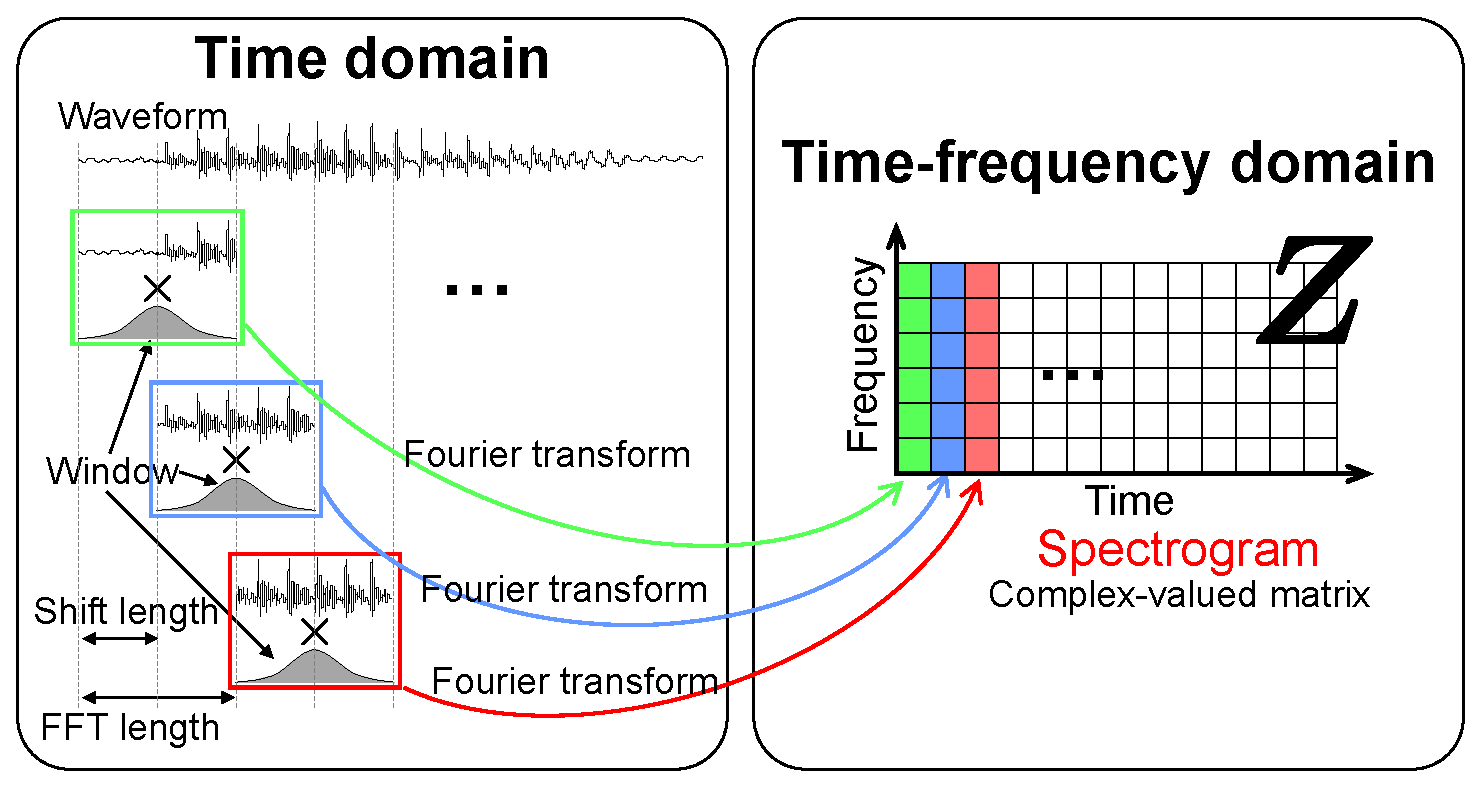
\includegraphics[width=0.95\columnwidth]{figures/stft.eps}
    \end{center}
    \vspace{-8pt}
	\caption{Mechanism of STFT.}
	\label{fig:stft}
\end{figure}
%%%%%%%%%%%%%%%%%%%%%%%%%%%%
STFTはFig.~\ref{fig:stft}に示すような時
間的に変化するスペクトルを表現するための手法である.
STFT の分析窓関数の長さ及びシフト長をそれぞれ$Q$及び$\tau$としたとき,時間領域の信号
$z(l)$の$j$番目の短時間区間(時間フレーム)の信号は次式で表される.
\begin{align}
    \bm{z}^{(j)} &= \left[z\left((j-1)\tau+1\right), z\left((j-1)\tau+2\right), \cdots , z\left((j-1)\tau+Q\right) \right]^{T}\\
    &= \left[
    z^{(j)}(1),z^{(j)}(2),\cdots , z^{(j)}(q), \cdots , z^{(j)}(Q)
    \right]^{T}~\in \mathbb{R}^{Q}
\end{align}
ここで,$j= 1, 2, \cdots , J$及び$q= 1, 2, \cdots , Q$は,それぞれ時間フレーム及び時間フレーム内のサン
プルを示す.また,セグメント数$J$は次式によって与えられる.
\begin{align}
    J = \frac{L}{\tau}
\end{align}
また,各時間フレームの信号のSTFTは次式のようにして求められる.
\begin{align}
\bm{Z}= {\rm STFT}_{\bm{\omega}}(\bm{z})~\in \mathbb{C}^{I \times J}
\end{align}
また,スペクトログラム$\bm{Z}$の$(i, j)$ 番目の要素は次式で表される.
\begin{align}
    z_{ij}= \sum_{q=1}^{Q}\omega(q)z^{(j)}(q){\rm exp}\left\{\frac{-\iota2\pi(q-1)(i-1)}{F}\right\}
\end{align}
ここで$F$は$\lfloor \frac{F}{2}\rfloor+1 =I$を満たす整数($\lfloor \cdot \rfloor$は床関数)を,$i= 1, 2, \cdots , I$は周波数ビンのインデクスを,
$\iota$は虚数単位を,$\bm{\omega}$は分析窓関数を示している.
このように,時間領域の信号は一定幅の短時間ごとに分析窓関数を乗じて離散フーリエ変換を行うことで,横軸が時間,縦軸が周波数のスペクトログラムと呼ばれる複素行列$\bm{Z}$で表すことができる.

%----------------------------------------------
\section{周波数領域におけるBSSの定式化}
\label{sec:formularization}
%----------------------------------------------
今一度,音源数と観測チャネル数(マイクロホン数)をそれぞれ$N$及び$M$とする.
また,各観測音源信号をSTFTすることで得られる,各時間周波数における音声信号,混合信号,及び分離信号をそれぞれ
\begin{align}
  \bm{s}_{ij} &= \left[
	s_{ij,1},s_{ij,2}, \cdots, s_{ij,n}, \cdots, s_{ij,N} 
  \right]^\mathrm{T}~\in \mathbb{C}^{N}\\
  \bm{x}_{ij} &= \left[
      x_{ij,1},x_{ij,2},  \cdots, x_{ij,m}, \cdots  , x_{ij,M} 
  \right]^\mathrm{T}~\in \mathbb{C}^{M} \\
  \bm{z}_{ij} &= \left[
      z_{ij,1},z_{ij,2},  \cdots, z_{ij,n}, \cdots  , z_{ij,N} 
  \right]^\mathrm{T}~\in \mathbb{C}^{N}
\end{align}
と表す.
ここで,$i= 1, 2, \cdots , I$,$j = 1, 2, \cdots , J$,$n = 1, 2, \cdots , N$,及び$m =
1, 2, \cdots , M $はそれぞれ周波数,時間,音源,チャネルのインデクスを示す.
また,複素スペクトログラム行列$\bm{S}_{n} \in \mathbb{C}^{I\times J}$, $\bm{X}_{m} \in \mathbb{C}^{I\times J}$及び$\bm{Z}_{n} \in \mathbb{C}^{I\times J}$の成分をそれぞれ
$s_{i, j, n}$, $x_{i, j, m}$及び$z_{i, j, n}$ と表す.

%----------------------------------------------
\section{FDICA}
\label{sec:fdica}
%----------------------------------------------
\ref{sec:ica}節で説明したように,ICAとは,観測信号が独立信号の線形結合として観測される場合に,各信号間の独立性を最も高めるように線形分離行列を推定することでBSSを実現する手法である.
しかし,実際に観測される音声信号には残響の影響を受けており,線形時不変なインパルス応答が畳み込まれて混合される.
インパルス応答の畳み込みは残響長$R$を用いて次式のように表される.
\begin{align}
  \bm{x}(l) = \sum_n \sum_{l^{'}=0}^{R-1} \tilde{\bm{a}}_n(l^{'}) \bm{s}_n(l-l^{'})
  \label{f:tatami}
\end{align}
ここで,$\tilde{\bm{a}}_n(l)$は,音源$n$に対する畳み込み混合係数ベクトル(音源$n$からマイクロフォン$m$までのインパルス応答をまとめたもの)である.
これを分離するためには逆畳み込みフィルタを推定することが必要となる.
一般的に逆畳み込みフィルタの推定は容易ではないことから,時間領域でのICAによるBSSは困難である.
この問題を解決するために,式(\ref{f:tatami})の時間領域における畳み込み混合を,STFTによって周波数領域上での瞬時混合に変換し,時間周波数領域で周波数毎にICAを行うFDICAが提案された.

FDICAでは,周波数毎の時不変な混合行列 $\bm{A}_{i} = (\bm{a}_{i, 1} ~\bm{a}_{i, 2} ~\cdots ~\bm{a}_{i, n}~\cdots,\bm{a}_{i, N} )\in \mathbb{C}^{M\times N}$を定義し,混合信号が次式で表現できると仮定する.
\begin{align}
 \bm{x}_{ij} = \bm{A}_i\bm{s}_{ij}
\end{align}
この混合モデルは,STFTの窓長が室内残響よりも長い場合にのみ成立する.
以後,決定的な系($M=N$)を仮定すると,混合行列$\bm{A}_{i}$が正則であれば,分離行列$\bm{W}_i=\bm{A}_i^{-1}=(\bm{w}_{i,1}~\bm{w}_{i,2}~ ...~ \bm{w}_{i, n}~ ... ~\bm{w}_{i, N})^{\mathrm{H}}$を用いて,分離信号を次式で表せる.
\begin{align}
 \bm{z}_{ij} = \bm{W}_{i}\bm{x}_{ij} \label{eq:sep}
\end{align}
ここで,$\cdot^\mathrm{H}$はベクトルや行列のエルミート転置を示す.
分離行列の行ベクトルである$\bm{w}_{i,n}\in\mathbb{C}^M$は,周波数$i$において,観測信号から$n$番目のみの音源へ変換する分離フィルタである.
このようにFDICAでは,観測信号$\bm{x}_{ij}$の各周波数ビンに対しそれぞれ独立にICA を適用することで,周波数毎の分離行列$\bm{W}_{i}$を全周波数にわたって推定することで音源分離を行う.

%----------------------------------------------
\section{パーミュテーション問題とその解決}
\label{sec:pp}
%----------------------------------------------
FDICA中で周波数毎に適用しているICAは,音源間の統計的独立性のみに基づいて分離行列を推定するため,分離音源の周波数毎のスケール及び順番に関しては不定である.
従って,FDICAの推定分離行列を$\hat{\bm{W}}_i$とすると,次式のような不定性が残る.
\begin{align}
	\hat{\bm{W}}_{i} &= \bm{D}_{i}\bm{P}_{i}  \bm{W}_{i}
\end{align}
ここで,$\bm{P}_i \in \{0, 1\}^{N \times N}$は分離行列$\bm{W}_{i}$の行ベクトル$\bm{w}_{i, n}$の順番を入れ変えうるパーミュテーション行列(置換行列)である.
$\bm{D}_i \in \mathbb{R}^{N \times N}$は,$\bm{w}_{i,n}$のスケールを変化させる可能性のある対角行列である.
即ち,FDICAで推定される分離信号
\begin{align}
\bm{y}_{ij} &= \hat{\bm{W}}_i\bm{x}_{ij} \\
&=\left[ y_{ij,1},y_{ij,2}, \cdots, y_{ij,n}, \cdots, y_{ij,N} \right]^\mathrm{T}~\in \mathbb{C}^{N} \label{eq:sepSig}
\end{align}
は,推定音源の順番やスケールが周波数毎にばらばらになっている状態である.
このうち,$\bm{D}_i$によって生じるスケールの任意性は,プロジェクションバック法\cite{Matsuoka2001_PB}で復元可能である.
一方で,$\bm{P}_i$によって生じる分離信号の順番の任意性(パーミュテーション)を純粋に復元することは,組み合わせ爆発が発生するため容易ではない.
この問題は,一般的にパーミュテーション問題と呼ばれる.
パーミュテーション問題の概要をFig.~\ref{fig:permu}に示す.
ここで,FDICAで推定される分離信号$\bm{y}_{ij}$の音源毎の複素スペクト
ログラム行列を$\bm{Y}_n \in \mathbb{C}^{I \times J}$で表している.
FDICA直後の$\bm{Y}_n$に注目すると,周波数毎での音源分離は達成できている.
しかし,時間周波数構造全体としては,異なるグループの分離信号が1つの時間周波数構造に混在していることが分かる.
これがパーミュテーション問題であり,ICAの分離信号の順番に関する不定性に起因して発生している.
そのため,FDICAにはポスト処理として,分離された音源の順番を全周波数ビンにわたって正しく並べ直す必要がある.
%%%%%%%%%%%%%%%%%%%%%%%%%%%%
\begin{figure}[t]
    \begin{center}
        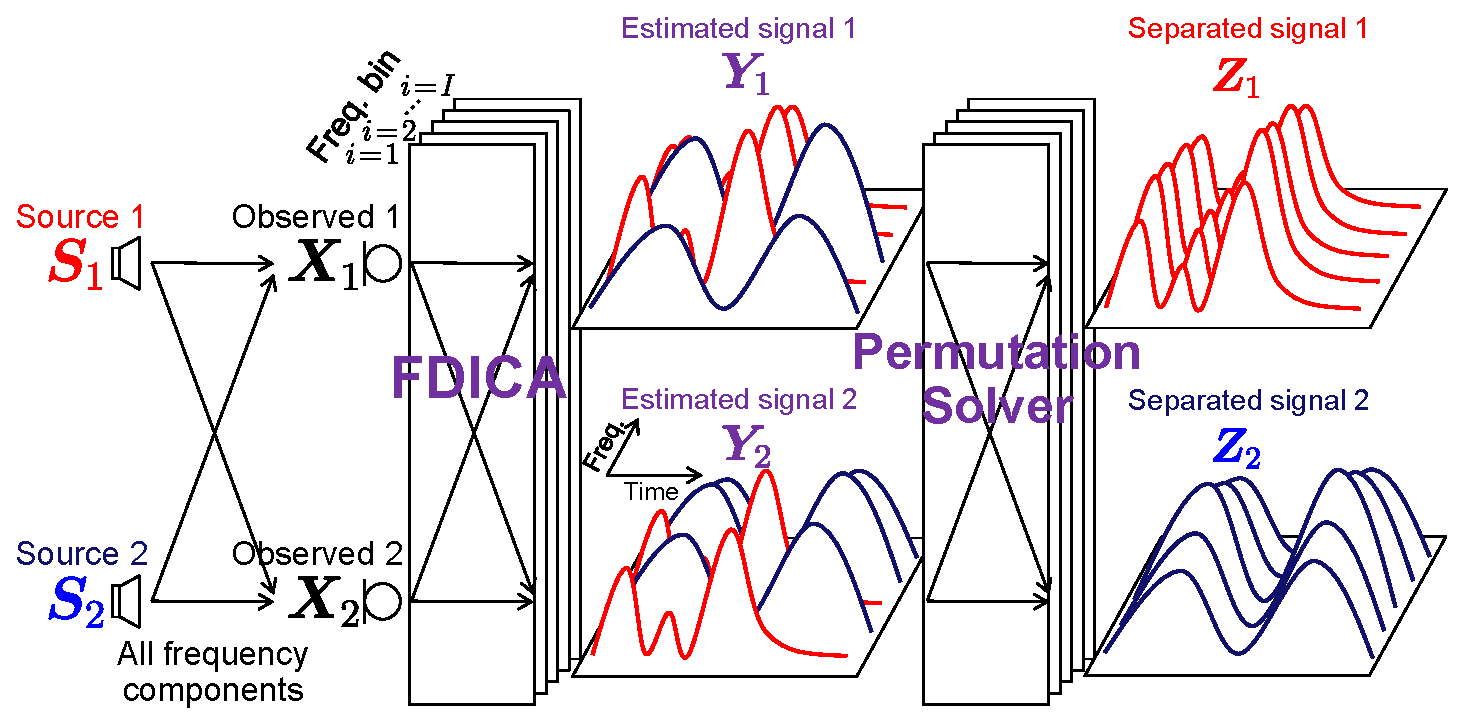
\includegraphics[width=0.95\columnwidth]{figures/permutation_image.eps}
    \end{center}
    \vspace{-8pt}
	\caption{Permutation problem in FDICA, where $N=M=2$.}
	\label{fig:permu}
\end{figure}
%%%%%%%%%%%%%%%%%%%%%%%%%%%%

パーミュテーション問題を解決して得られる分離信号は次式となる.
\begin{align}
\bm{z}_{ij} &= \bm{P}_{i}^{-1}\bm{D}_{i}^{-1}\bm{y}_{ij} \label{eq:z}
\end{align}
%本論文では,この$\bm{P}_{i}^{-1}$を推定することが目的となる.

このパーミュテーション問題を解決するために,これまでにも数々のパーミュテーション解決法が提案されてきた.
代表的な既存手法の1つに,隣接周波数の時系列強度(音源アクティベーション)の相関を用いたパーミュテーション解決法\cite{COR}がある.
これは,分離信号のパーミュテーションが正しければ,隣接した周波数アクティベーション間の相関が高くなりやすいという仮定の下で並べ替える手法である.また,離れた周波数においても,同じ音源のアクティベーション間の相関が高くなるように並び替えられている.
%り,次式のように相関を計算する.
%\begin{align}
%\Tilde{\bm{v}}_{i}(n) &=  \frac{1}{J}\sum_{j=0}^{J} |\bm{y}_{i,j,n}| \\
% {\rm sim}(i) &= \sum_{n\neq m} \frac{\Tilde{\bm{v}}_{i}(n) \cdot \Tilde{\bm{v}}_{i}(m)}{\|
% \Tilde{\bm{v}}_{i}(n)\|~\| \Tilde{\bm{v}}_{i}(m)\|}
%\end{align}
%ここで,$\cdot$は内積を表しており,
他にも,マイクロホンの相対的な位置情報を既知として音源到来方位を計算し,パーミュテーション解決の手掛かりとする手法 \cite{DOA}及び両者を組み合わせたパーミュテーション解決法も提案されている.
しかしながら,パーミュテーション問題の解は組み合わせ爆発を起こすことから,上記いずれの手法を用
いても完璧にパーミュテーション問題を解くことは非常に難しく,とくに複数音声の混合信号における高精
度なパーミュテーション問題の解決はいまだできていない.

%----------------------------------------------
\section{IVAとILRMA}
\label{sec:ivailrma}
%----------------------------------------------



FDICA に対して音源の時間周波数成分の共起関係を新たに仮定して,パーミュテーション問題を回避しつつ分離信号を推定する手法が登場している.
例えば,IVA~\cite{IVA1,IVA2}は,同一音源の周波数成分の共起を仮定
しており,FDICAでは周波数毎に独立性を最大化していたのに対し,IVAでは全周波数成分をまとめてベクトル変数とし,べクトル間の独立性を最大化するようなモデルとなっている.
そのため同じ音源の分離信号は全周波数でまとめて出力されるような分離モデルとなっており.パーミュテーション問題を回避することが期待できる.
また,NMF~\cite{NMF}とIVAを組み合わせたBSSであるILRMA~\cite{ILRMA1,ILRMA2} は,同一音源の時間周波数成分の共起が低ランク構造を持つことを仮定
しており,IVAと同様にパーミュテーション問題を音源モデルに基づいて可能な限り回避するようなモデルとなっている.

%%%%%%%%%%%%%%%%%%%%%%%%%%%%
\begin{figure}[t]
  \begin{center}
      \includegraphics[width=0.95\columnwidth]{figures/block_perm_example.eps}
  \end{center}
  \vspace{-8pt}
\caption{Example of block permutation problem.}
\label{fig:bp}
\end{figure}
%%%%%%%%%%%%%%%%%%%%%%%%%%%%

しかし,音声と音声の混合信号の様な分離タスクの場合,IVAやILRMAを用いてもしばしば分離に失敗してしまう.
これは,音声信号の時間周波数成分がダイナミックに変動することから,音声信号のパワースペクトログラムを低ランクで表現することが難しいことが原因と予想される.
また,IVAやILRMAにおいても,まとまった周波数帯域でパーミュテーションが入れ替わる問題(ブロックパーミュテーション問題)\cite{brock_p}が報告されている.
Fig.~\ref{fig:bp}にブロックパーミュテーション問題の様子を示す.
Fig.~\ref{fig:bp}では,$4000$hz以上の周波数帯がまとめて反転していることが分かる.
そのため,依然としてパーミュテーション問題の解決が不十分であることが分かる.


%----------------------------------------------
\section{深層パーミュテーション解決法}
\label{sec:DNNs}
%----------------------------------------------

近年では,DNNを用いたパーミュテーション問題解決法が登場している.観測された混合信号$\bm{X}_n$にFDICA適用すると,パーミュテーション問題が生じた分離信号$\bm{Y}_n$が得られる.
これらのパワースペクトログラム$|\bm{Y}_n|^{.2}$から全周波数帯域中の局所的な狭帯域(サブバンド)を定義し,サブバンド毎にデータをDNNに入力し,パーミュテーション問題を解決する.
サブバンド毎に参照周波数を定義し,その近傍周波数が参照周波数に対して同一音源か否かを判断し,同一音源である場合はDNNの出力として「0」を出力し,同一音源でない場合はDNNの出力として「1」を出力する.

この結果を時間方向にずらして,全時間フレームに対するDNNの予測処理を走査する.そして,DNNの予測結果を時間方向に対して多数決処理を行うことで,より信頼性の高いサブバンドベクトルを取得する.
サブバンドベクトルは,基準周波数$i$をシフトすることにより全周波数を推定する.ただ,各サブバンドベクトル内の2値は(「0」及び「1」)は異なる意味を持つ可能性がある.これはサブバンド内の周波数成分が.
参照周波数の成分と同一音源か否かを示しているに過ぎず,参照周波数の変化を共に,対応音源が変化する.2音源の場合を考えるとサブバンドベクトル内の値が「1」,つまり同一音源ではない時,必然的にもう一方の音源を指すこととなる.
但し,3音源以上になるとサブバンドベクトル内の値が「1」の時,残りのどの音源のことを指すのかが判断できない.
3音源以上になると組み合せ爆発を起こしてしまい,計算量の観点から3音源以上の音源分離は難しい.

%----------------------------------------------
\section{本章のまとめ}
%----------------------------------------------
本章では,提案手法において必要となる基礎理論及び各種従来手法について説明した.
次章以降では,より簡潔に精度の良いBSSを達成するために\ref{sec:fdica}節で導入したFDICAのポスト処理として,DNNに基づくパーミュテーション解決法を新たに提案する.
















